%!TEX program = xelatex
%!TEX root = ../all.tex
\chapter{Cooccurrence Data and Latent Semantic Methods}

\section*{Exploiting Co-occurrence Data: Motivation and Framework}

The analysis of co-occurrence patterns represents a fundamental paradigm in modern machine learning and data mining, with applications spanning text analysis, recommender systems, social network analysis, and beyond. At its core, the co-occurrence framework seeks to extract meaningful structure from observations of how entities from two different collections appear together. The ubiquity of this pattern across domains reflects a deep principle: relationships between entities are often most naturally expressed not through direct measurements of the entities themselves, but through observations of their joint occurrences in particular contexts.

Consider, for example, the relationship between terms and documents in a text corpus. While we could attempt to characterize each term or document in isolation, much of the semantic information we seek is actually encoded in the pattern of which terms appear in which documents. A term like "photosynthesis" acquires its meaning not from any intrinsic property, but from its tendency to co-occur with other biology-related terms in scientific documents. Similarly, in recommender systems, the relationship between customers and products is revealed through purchasing or browsing patterns—co-occurrences of customers accessing item descriptions. In social networks, the structure of relationships emerges from patterns of interaction between people.

More formally, models addressing co-occurrence data begin with two finite collections, which we denote generically as $\mathcal{V}$ and $\mathcal{D}$. The interpretation of these sets depends on the application domain: they might represent terms and documents in text analysis, customers and items in e-commerce, or users and resources in a web platform. The fundamental data consists of a sequence of observations $\mathcal{W} = \{(w_1, d_1), \ldots, (w_N, d_N)\}$, where each observation records a co-occurrence event with $w_i \in \mathcal{V}$ and $d_i \in \mathcal{D}$. In the text domain, these observations correspond to individual occurrences of terms within documents; in e-commerce, they might represent instances of customers viewing or purchasing items; in social networks, they capture interaction events between pairs of people.

The central computational challenges and opportunities presented by co-occurrence data are twofold. First, we seek to derive meaningful notions of similarity between entities—both within a single collection (term-to-term similarity, document-to-document similarity) and across collections (term-to-document relevance). These similarity measures enable clustering, classification, and retrieval tasks. Second, we aim to make predictions about future observations or unobserved co-occurrences, such as predicting which products a customer might be interested in based on their past behavior and the behavior of similar customers.

The approach we will explore in detail, known as Latent Semantic Analysis (LSA), rests on three foundational assumptions that deserve careful consideration. First, LSA posits that semantic information—the meaningful relationships and conceptual structure underlying the observations—can be derived from the matrix of term-document co-occurrences, even though this matrix contains only frequency counts rather than explicit semantic annotations. This assumption reflects a distributional hypothesis: entities that co-occur in similar contexts tend to be semantically related. Second, LSA asserts that dimensionality reduction is not merely a computational convenience but a key aspect of semantic extraction. The reasoning is that the raw co-occurrence matrix is both high-dimensional and sparse, containing substantial noise alongside the signal we wish to extract. By projecting into a lower-dimensional space, we can filter noise and reveal the dominant latent structure. Third, LSA assumes that both terms and documents can be meaningfully modeled as points or vectors in a Euclidean space, allowing us to apply geometric notions of distance and similarity.

To make these ideas concrete, let us establish the basic mathematical framework. We begin with a dictionary $\mathcal{V}$ containing $V = |\mathcal{V}|$ distinct terms, which we denote $t_1, t_2, \ldots, t_V$. This vocabulary might consist of all words appearing in a text collection (possibly after preprocessing such as stemming and stop word removal), or more generally, any set of discrete entities we wish to analyze. We also have a corpus $\mathcal{D}$ consisting of $D = |\mathcal{D}|$ documents, denoted $d_1, d_2, \ldots, d_D$. Each document $d_i$ is conceptualized as a sequence of $N_i$ term occurrences drawn from the vocabulary $\mathcal{V}$.

A crucial modeling decision in LSA is the adoption of the bag-of-words hypothesis, borrowed from information retrieval. Under this assumption, a document $d_i$ is treated not as an ordered sequence of terms preserving syntactic structure, but rather as a multiset—an unordered collection where terms may appear with multiplicity but position and ordering are discarded. This simplification, while clearly losing information about word order and grammar, has proven remarkably effective for many semantic tasks. The assumption can be justified both pragmatically (it dramatically simplifies the mathematical framework) and theoretically (through notions of exchangeability that we will discuss later).

Given these modeling choices, we postulate the existence of a correspondence between the sets $\mathcal{V}$ and $\mathcal{D}$ and a vector space $\mathcal{S}$. More specifically, LSA seeks to associate with each term $t_i$ a vector $\mathbf{u}_i \in \mathcal{S}$, and with each document $d_j$ a vector $\mathbf{v}_j \in \mathcal{S}$. The geometry of this space—the distances and angles between vectors—will encode semantic relationships: terms with similar meanings will have nearby vector representations, as will semantically related documents.

The bridge connecting the discrete co-occurrence observations to this continuous vector space representation is the occurrence matrix, which we denote $\mathbf{W} \in \mathbb{R}^{V \times D}$. The entry $w_{i,j}$ of this matrix quantifies the association between term $t_i$ and document $d_j$, and it can be derived from various measures of occurrence strength. The simplest choice is a binary indicator (1 if term $t_i$ appears anywhere in document $d_j$, 0 otherwise), but in practice, we often use more sophisticated weighting schemes. Raw term frequency counts the number of times $t_i$ occurs in $d_j$, capturing not just presence but intensity of usage. The term frequency-inverse document frequency (TF-IDF) weighting adjusts raw counts to down-weight terms that appear in many documents and are therefore less discriminative. Other schemes based on entropy or statistical measures are also employed depending on the application.

The structure of the occurrence matrix $\mathbf{W}$ reveals important aspects of the representation. Each row of $\mathbf{W}$ corresponds to a single term, represented as a vector of length $D$. Crucially, this representation is entirely defined by which documents contain the term and how strongly it appears in each—there is no external semantic annotation. The term's meaning is purely distributional, derived from its pattern of co-occurrence with documents. Symmetrically, each column of $\mathbf{W}$ corresponds to a document, represented as a vector of length $V$. Again, the document's representation is defined solely by its constituent terms and their weights—the document is nothing more than its word distribution.

This representation, while conceptually elegant, presents significant practical challenges that motivate the dimensionality reduction approach at the heart of LSA. First, the dimensions $V$ and $D$ are typically very large. A moderately-sized text collection might contain tens of thousands of unique terms and thousands of documents, yielding matrices with millions or tens of millions of entries. Second, despite this high dimensionality, the vectors are extremely sparse. Most terms appear in only a small fraction of documents, so the overwhelming majority of entries in $\mathbf{W}$ are zero. This sparsity wastes representational capacity and makes distance computations unreliable. Third, there is a fundamental asymmetry in the representation: terms are modeled as vectors in $\mathbb{R}^D$ while documents are modeled as vectors in $\mathbb{R}^V$. These are different spaces with different dimensions, preventing direct comparison of term vectors to document vectors.

The solution to these challenges, and the mathematical foundation of LSA, is the Singular Value Decomposition—a powerful matrix factorization technique that will allow us to project both terms and documents into a common, lower-dimensional semantic space where meaningful structure can be revealed and noise filtered away. Before turning to the application of SVD in the LSA framework, we must first develop a thorough understanding of the SVD itself, including its mathematical properties, geometric interpretation, and computational aspects.

\subsection*{Introduction to Singular Value Decomposition}

The Singular Value Decomposition stands as one of the most important and widely applicable tools in modern linear algebra and numerical analysis. Its power derives from a remarkable fact: any real matrix, regardless of its properties—whether square or rectangular, symmetric or asymmetric, full rank or rank deficient—admits a canonical factorization that reveals its fundamental structure. This decomposition provides insight into the geometry of linear transformations, enables optimal low-rank approximations, and forms the computational backbone of numerous algorithms in machine learning, signal processing, and scientific computing.

Let $\mathbf{W} \in \mathbb{R}^{n \times m}$ be a real matrix of rank $r \leq \min(n,m)$, and assume without loss of generality that $n > m$. (The case $m > n$ can be handled by considering $\mathbf{W}^T$ instead.) Our goal is to derive, in a constructive and rigorous manner, the Singular Value Decomposition of $\mathbf{W}$, namely a factorization of the form:
\begin{myequation}
\mathbf{W} = \mathbf{U} \boldsymbol{\Sigma} \mathbf{V}^T
\end{myequation}
where the matrices $\mathbf{U}$, $\boldsymbol{\Sigma}$, and $\mathbf{V}$ possess precise algebraic and geometric properties that we will establish through careful construction.

More specifically, we will demonstrate the existence of three matrices satisfying the following conditions. First, there exists a matrix $\mathbf{U} \in \mathbb{R}^{n \times r}$ whose columns form an orthonormal set of vectors. This orthonormality condition can be expressed compactly as $\mathbf{U}^T \mathbf{U} = \mathbf{I}_r$, where $\mathbf{I}_r$ denotes the $r \times r$ identity matrix. The columns of $\mathbf{U}$ are called the left singular vectors of $\mathbf{W}$. Second, there exists a matrix $\mathbf{V} \in \mathbb{R}^{m \times r}$ whose columns also form an orthonormal set, satisfying $\mathbf{V}^T \mathbf{V} = \mathbf{I}_r$. The columns of $\mathbf{V}$ are the right singular vectors. Third, there exists a diagonal matrix $\boldsymbol{\Sigma} \in \mathbb{R}^{r \times r}$ with strictly positive diagonal entries $\sigma_1, \sigma_2, \ldots, \sigma_r$, conventionally ordered in non-increasing order: $\sigma_1 \geq \sigma_2 \geq \cdots \geq \sigma_r > 0$. These diagonal values are called the singular values of $\mathbf{W}$.

The decomposition can be visualized schematically as the product of three simpler matrices with well-defined geometric interpretations. The visual representation helps build intuition: the original $n \times m$ matrix $\mathbf{W}$ is factored as the product of a tall, thin orthonormal matrix $\mathbf{U}$ (dimension $n \times r$), a small diagonal matrix $\boldsymbol{\Sigma}$ (dimension $r \times r$), and a wide, thin orthonormal matrix $\mathbf{V}^T$ (dimension $r \times m$).

\begin{figure}
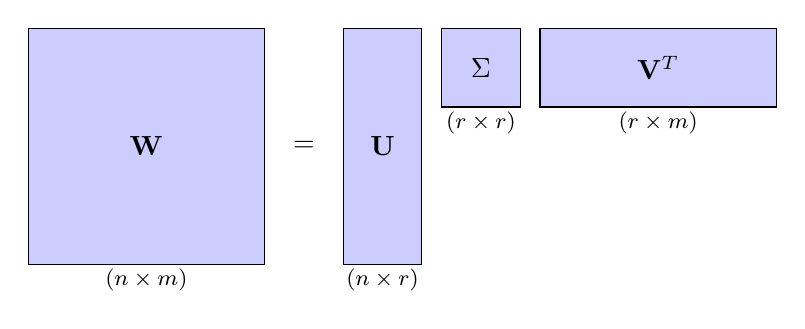
\begin{tikzpicture}[fill=blue!20, every path/.style={draw}]
\fill (-1,0) rectangle +(3,3);
\node (a) at (.5,1.5) {$\mathbf{W}$};
\node (d) at (2.5,1.5) {=};
\fill (3,0) rectangle +(1,3);
\node (e) at (3.5,1.5) {$\mathbf{U}$};
\fill (4.25,2) rectangle +(1,1);
\node (f) at (4.75,2.5) {$\boldsymbol{\Sigma}$};
\fill (5.5,2) rectangle +(3,1);
\node (g) at (7,2.5) {$\mathbf{V}^{T}$};
\node (h) at (.5,-0.2) {\footnotesize$(n\times m)$};
\node (i) at (3.5,-0.2) {\footnotesize$(n\times r)$};
\node (l) at (4.75,1.8) {\footnotesize$(r\times r)$};
\node (m) at (7,1.8) {\footnotesize$(r\times m)$};
\end{tikzpicture}
\end{figure}

\subsection*{Constructing the SVD: A Detailed Derivation}

The construction of the Singular Value Decomposition proceeds through a sequence of carefully orchestrated steps, beginning with an auxiliary matrix that encodes essential spectral information about $\mathbf{W}$. This construction is not merely a mathematical curiosity—it provides computational algorithms for computing the SVD and reveals deep connections to eigenvalue problems and optimization.

We begin by forming the Gram matrix:
\begin{myequation}
\mathbf{A} = \mathbf{W}^T \mathbf{W} \in \mathbb{R}^{m \times m}
\end{myequation}

This matrix plays a central role in our construction, as it encodes all the information needed to recover the right singular vectors and singular values of $\mathbf{W}$. To understand why $\mathbf{A}$ is so informative, we must first establish its fundamental properties.

Several key properties of $\mathbf{A}$ follow immediately from its construction. First, the rank of $\mathbf{A}$ equals the rank of $\mathbf{W}$: $\text{rank}(\mathbf{A}) = \text{rank}(\mathbf{W}) = r$. This equality reflects the fact that $\mathbf{A}$ captures the essential structure of $\mathbf{W}$ despite being a smaller matrix. Second, the matrix $\mathbf{A}$ is symmetric. To see this, write $\mathbf{W}$ in terms of its column vectors: $\mathbf{W} = [\mathbf{w}_1 \ \mathbf{w}_2 \ \cdots \ \mathbf{w}_m]$. Then the $(i,j)$ entry of $\mathbf{A}$ is:
\begin{myequation}
a_{ij} = \mathbf{w}_i^T \mathbf{w}_j = \mathbf{w}_j^T \mathbf{w}_i = a_{ji}
\end{myequation}
demonstrating symmetry. Third, and most importantly, $\mathbf{A}$ is positive semidefinite. For any nonzero vector $\mathbf{x} \in \mathbb{R}^m$, we have:
\begin{myequation}
\mathbf{x}^T \mathbf{A} \mathbf{x} = \mathbf{x}^T \mathbf{W}^T \mathbf{W} \mathbf{x} = (\mathbf{W}\mathbf{x})^T (\mathbf{W}\mathbf{x}) = \|\mathbf{W}\mathbf{x}\|_2^2 \geq 0
\end{myequation}

This inequality establishes positive semidefiniteness, which has profound implications for the spectral properties of $\mathbf{A}$.

Because $\mathbf{A}$ is a real symmetric matrix, the fundamental spectral theorem of linear algebra applies in its full strength. This theorem guarantees that all eigenvalues of $\mathbf{A}$ are real numbers (as opposed to complex), and that $\mathbf{A}$ admits a complete orthonormal basis of eigenvectors. These properties are not obvious a priori, and their proof requires careful use of the symmetry assumption.

To establish that eigenvalues are real, suppose $\lambda \in \mathbb{C}$ is an eigenvalue of $\mathbf{A}$ with corresponding eigenvector $\mathbf{v} \in \mathbb{C}^m$, $\mathbf{v} \neq \mathbf{0}$. By definition:
\begin{myequation}
\mathbf{A} \mathbf{v} = \lambda \mathbf{v}
\end{myequation}

Taking the conjugate transpose of both sides and using the symmetry of $\mathbf{A}$ (which implies $\mathbf{A}$ equals its conjugate transpose), we obtain:
\begin{myequation}
\overline{\mathbf{v}}^T \mathbf{A} \mathbf{v} = \lambda \overline{\mathbf{v}}^T \mathbf{v}
\end{myequation}

On the other hand, since the conjugate of an eigenvalue-eigenvector pair is also an eigenvalue-eigenvector pair for a real symmetric matrix, we have:
\begin{myequation}
\overline{\mathbf{v}}^T \mathbf{A} \mathbf{v} = \overline{\lambda} \overline{\mathbf{v}}^T \mathbf{v}
\end{myequation}

Subtracting these two expressions yields:
\begin{myequation}
(\lambda - \overline{\lambda}) \|\mathbf{v}\|^2 = 0
\end{myequation}

Since $\mathbf{v} \neq \mathbf{0}$, we must have $\lambda = \overline{\lambda}$, which means $\lambda \in \mathbb{R}$—the eigenvalue is real.

Moreover, eigenvectors corresponding to distinct eigenvalues are necessarily orthogonal. To see this, suppose:
\begin{myequation}
\mathbf{A}\mathbf{v}_1 = \lambda_1 \mathbf{v}_1, \quad \mathbf{A}\mathbf{v}_2 = \lambda_2 \mathbf{v}_2
\end{myequation}
with $\lambda_1 \neq \lambda_2$. Then:
\begin{myequation}
\lambda_1 \mathbf{v}_1^T \mathbf{v}_2 = (\mathbf{A}\mathbf{v}_1)^T \mathbf{v}_2 = \mathbf{v}_1^T \mathbf{A} \mathbf{v}_2 = \lambda_2 \mathbf{v}_1^T \mathbf{v}_2
\end{myequation}

This implies $(\lambda_1 - \lambda_2) \mathbf{v}_1^T \mathbf{v}_2 = 0$. Since $\lambda_1 \neq \lambda_2$ by assumption, we must have $\mathbf{v}_1^T \mathbf{v}_2 = 0$—the eigenvectors are orthogonal.

The positive semidefiniteness of $\mathbf{A}$ provides an additional crucial property: all its eigenvalues are nonnegative. For any eigenpair $(\lambda, \mathbf{v})$ with $\mathbf{v} \neq \mathbf{0}$:
\begin{myequation}
\lambda = \frac{\mathbf{v}^T \mathbf{A} \mathbf{v}}{\|\mathbf{v}\|^2} \geq 0
\end{myequation}

where the inequality follows from the positive semidefiniteness established earlier. As a consequence of rank considerations, $\mathbf{A}$ has exactly $r$ strictly positive eigenvalues:
\begin{myequation}
\lambda_1, \lambda_2, \ldots, \lambda_r > 0
\end{myequation}
with associated orthonormal eigenvectors $\mathbf{v}_1, \mathbf{v}_2, \ldots, \mathbf{v}_r$. These eigenvectors can be chosen to satisfy $\|\mathbf{v}_i\| = 1$ and $\mathbf{v}_i^T \mathbf{v}_j = 0$ for $i \neq j$.

Having established the spectral properties of $\mathbf{A}$, we now use these eigenvalues and eigenvectors to construct the components of the SVD. We define the singular values of $\mathbf{W}$ as the square roots of the eigenvalues of $\mathbf{A}$:
\begin{myequation}
\sigma_i = \sqrt{\lambda_i}, \quad i = 1, \ldots, r
\end{myequation}

This definition ensures that singular values are positive real numbers. Next, we introduce the left singular vectors through the formula:
\begin{myequation}
\mathbf{u}_i = \frac{1}{\sigma_i} \mathbf{W} \mathbf{v}_i, \quad i = 1, \ldots, r
\end{myequation}

These vectors are well-defined because $\sigma_i > 0$ for all $i \leq r$, and they possess remarkable properties. First, they are orthonormal. To verify this, consider:
\begin{myequation}
\mathbf{u}_i^T \mathbf{u}_j = \frac{1}{\sigma_i \sigma_j} \mathbf{v}_i^T \mathbf{W}^T \mathbf{W} \mathbf{v}_j = \frac{1}{\sigma_i \sigma_j} \mathbf{v}_i^T (\lambda_j \mathbf{v}_j) = \frac{\sigma_j}{\sigma_i} \mathbf{v}_i^T \mathbf{v}_j
\end{myequation}

This expression vanishes whenever $i \neq j$ because the eigenvectors $\mathbf{v}_i$ are orthogonal. Moreover:
\begin{myequation}
\|\mathbf{u}_i\|^2 = \frac{1}{\lambda_i} (\mathbf{W}\mathbf{v}_i)^T (\mathbf{W}\mathbf{v}_i) = \frac{1}{\lambda_i} \mathbf{v}_i^T (\mathbf{W}^T \mathbf{W} \mathbf{v}_i) = \frac{1}{\lambda_i} \mathbf{v}_i^T (\lambda_i \mathbf{v}_i) = 1
\end{myequation}

confirming that each $\mathbf{u}_i$ is a unit vector.

We now collect these vectors into matrices to express the SVD concisely. Define $\mathbf{V} \in \mathbb{R}^{m \times r}$ as the matrix whose columns are the right singular vectors:
\begin{myequation}
\mathbf{V} = [\mathbf{v}_1 \ \mathbf{v}_2 \ \cdots \ \mathbf{v}_r]
\end{myequation}

Similarly, define $\mathbf{U} \in \mathbb{R}^{n \times r}$ as the matrix whose columns are the left singular vectors:
\begin{myequation}
\mathbf{U} = [\mathbf{u}_1 \ \mathbf{u}_2 \ \cdots \ \mathbf{u}_r]
\end{myequation}

Finally, define $\boldsymbol{\Sigma} \in \mathbb{R}^{r \times r}$ as the diagonal matrix of singular values:
\begin{myequation}
\boldsymbol{\Sigma} = \begin{pmatrix}
\sigma_1 & 0 & \cdots & 0 \\
0 & \sigma_2 & \cdots & 0 \\
\vdots & \vdots & \ddots & \vdots \\
0 & 0 & \cdots & \sigma_r
\end{pmatrix}
\end{myequation}

By construction, we have the fundamental relation:
\begin{myequation}
\mathbf{W} \mathbf{V} = \mathbf{U} \boldsymbol{\Sigma}
\end{myequation}

To see this, observe that the $i$-th column of $\mathbf{W}\mathbf{V}$ is $\mathbf{W}\mathbf{v}_i$, while the $i$-th column of $\mathbf{U}\boldsymbol{\Sigma}$ is $\sigma_i \mathbf{u}_i = \sigma_i \cdot \frac{1}{\sigma_i} \mathbf{W}\mathbf{v}_i = \mathbf{W}\mathbf{v}_i$, confirming equality column by column.

Since $\mathbf{V}$ has orthonormal columns, $\mathbf{V}^T \mathbf{V} = \mathbf{I}_r$, we can multiply both sides of the above relation on the right by $\mathbf{V}^T$ to obtain:
\begin{myequation}
\mathbf{W} = \mathbf{U} \boldsymbol{\Sigma} \mathbf{V}^T
\end{myequation}

This is precisely the Singular Value Decomposition we sought to establish. The construction reveals that the SVD can be computed by finding the eigendecomposition of $\mathbf{W}^T \mathbf{W}$, providing both theoretical insight and a practical computational pathway.

\subsection*{Connection to Principal Component Analysis}

The Singular Value Decomposition is intimately connected to Principal Component Analysis, one of the most widely used dimensionality reduction techniques in statistics and machine learning. Understanding this connection not only provides geometric insight into SVD but also shows how PCA can be efficiently computed using SVD rather than through direct eigendecomposition of the covariance matrix.

Consider a data matrix $\mathbf{X} \in \mathbb{R}^{d \times n}$ containing $n$ observations of $d$-dimensional feature vectors. Each column of $\mathbf{X}$ represents a single data point. Before applying PCA, we center the data by subtracting the sample mean from each observation. This centering operation can be expressed in matrix form as:
\begin{myequation}
\tilde{\mathbf{X}} = \mathbf{X} \left( \mathbf{I} - \frac{1}{n} \mathbf{1} \mathbf{1}^T \right)
\end{myequation}
where $\mathbf{1} \in \mathbb{R}^n$ denotes the vector of all ones, and $\mathbf{I}$ is the $n \times n$ identity matrix. The matrix $\left(\mathbf{I} - \frac{1}{n}\mathbf{1}\mathbf{1}^T\right)$ is the centering operator: it projects each column onto the subspace orthogonal to $\mathbf{1}$, effectively subtracting the mean.

The scatter matrix, which plays a central role in PCA, is defined as:
\begin{myequation}
\mathbf{S} = \tilde{\mathbf{X}} \tilde{\mathbf{X}}^T
\end{myequation}

This matrix is proportional to the sample covariance matrix (the covariance is $\frac{1}{n-1}\mathbf{S}$ or $\frac{1}{n}\mathbf{S}$ depending on convention). Principal components are defined as the eigenvectors of $\mathbf{S}$, and the variance explained by each component is given by the corresponding eigenvalue.

Now suppose we compute the SVD of the centered data matrix:
\begin{myequation}
\tilde{\mathbf{X}} = \mathbf{U} \boldsymbol{\Sigma} \mathbf{V}^T
\end{myequation}
where $\mathbf{U} \in \mathbb{R}^{d \times d}$ and $\mathbf{V} \in \mathbb{R}^{n \times n}$ are orthogonal matrices satisfying $\mathbf{U}^T \mathbf{U} = \mathbf{I}$ and $\mathbf{V}^T \mathbf{V} = \mathbf{I}$, and $\boldsymbol{\Sigma} \in \mathbb{R}^{d \times n}$ is a diagonal matrix whose nonzero entries $\sigma_1, \ldots, \sigma_d$ are the singular values.

Using this SVD, we can express the scatter matrix as:
\begin{myequation}
\mathbf{S} = \tilde{\mathbf{X}} \tilde{\mathbf{X}}^T = (\mathbf{U} \boldsymbol{\Sigma} \mathbf{V}^T)(\mathbf{U} \boldsymbol{\Sigma} \mathbf{V}^T)^T = \mathbf{U} \boldsymbol{\Sigma} \mathbf{V}^T \mathbf{V} \boldsymbol{\Sigma}^T \mathbf{U}^T = \mathbf{U} \boldsymbol{\Sigma} \boldsymbol{\Sigma}^T \mathbf{U}^T
\end{myequation}

Since $\boldsymbol{\Sigma} \boldsymbol{\Sigma}^T$ is diagonal (with diagonal entries $\sigma_i^2$), this demonstrates that $\mathbf{S}$ admits the spectral decomposition:
\begin{myequation}
\mathbf{S} = \mathbf{U} \boldsymbol{\Lambda} \mathbf{U}^T, \quad \boldsymbol{\Lambda} = \boldsymbol{\Sigma} \boldsymbol{\Sigma}^T
\end{myequation}

The diagonal entries of $\boldsymbol{\Lambda}$ are $\sigma_1^2, \ldots, \sigma_d^2$, revealing that the eigenvalues of the scatter matrix $\mathbf{S}$ are precisely the squares of the singular values of the centered data matrix $\tilde{\mathbf{X}}$. Moreover, the corresponding eigenvectors—the principal components—are given by the columns of $\mathbf{U}$, which are the left singular vectors of $\tilde{\mathbf{X}}$.

This observation establishes a fundamental computational insight: to perform Principal Component Analysis on a data matrix $\mathbf{X}$, it is sufficient to compute the SVD of the centered matrix $\tilde{\mathbf{X}}$. The principal components are the columns of $\mathbf{U}$, and the variance explained by each component is given by the corresponding squared singular value $\sigma_i^2$. This approach is often numerically more stable and efficient than forming and eigendecomposing the scatter matrix $\mathbf{S}$ directly, especially when the data dimension is large.

\subsection*{Latent Semantic Analysis: Applying SVD to Text}

Having developed a thorough understanding of the Singular Value Decomposition and its properties, we now turn to its application in the domain of text analysis through Latent Semantic Analysis. LSA represents a seminal application of SVD outside pure numerical linear algebra, demonstrating how matrix factorization can extract semantic structure from discrete co-occurrence data.

The setting for LSA involves two finite collections: a vocabulary $\mathcal{V}$ and a document collection $\mathcal{D}$. The vocabulary might consist of all words appearing in a text corpus (after preprocessing), while the documents might be news articles, scientific papers, web pages, or any other text units. More generally, this framework extends beyond text: $\mathcal{V}$ and $\mathcal{D}$ could represent customers and products in e-commerce, users and resources in web platforms, or any two types of entities whose co-occurrence patterns we wish to analyze.

We observe a sequence of co-occurrence events:
\begin{myequation}
\mathcal{W} = \{(w_1, d_1), \ldots, (w_N, d_N)\}
\end{myequation}
where each $w_i \in \mathcal{V}$ and each $d_i \in \mathcal{D}$. In the text domain, each observation corresponds to a single occurrence of a specific term in a specific document. If a term appears multiple times in a document, there will be multiple observations recording this fact. The total number of observations $N$ equals the total number of term occurrences across the entire corpus.

The fundamental assumption underlying LSA is that semantic relationships between terms and between documents are implicitly encoded in these co-occurrence patterns, even though we never explicitly annotate documents with semantic labels or provide the system with a dictionary of word meanings. This assumption rests on the distributional hypothesis from linguistics: words that occur in similar contexts tend to have similar meanings, and documents that use similar vocabularies tend to discuss similar topics.

The LSA methodology rests on three key pillars. First, semantic relationships can be inferred from the statistical structure of co-occurrences. Terms that frequently appear together, or that appear in similar sets of documents, are likely to be semantically related. Second, dimensionality reduction is essential to reveal this latent structure. The raw co-occurrence matrix is high-dimensional, sparse, and noisy. By projecting into a lower-dimensional space, we filter noise and uncover the dominant patterns—the latent semantic dimensions. Third, both terms and documents can be meaningfully represented as vectors in a common Euclidean space. This geometric representation allows us to define similarity through distance or angle, enabling clustering, classification, and retrieval.

\subsection*{The Data Representation Framework}

Let us formalize the data representation. We have a dictionary $\mathcal{V} = \{t_1, t_2, \ldots, t_V\}$ of $V$ distinct terms, and a corpus $\mathcal{D} = \{d_1, d_2, \ldots, d_D\}$ of $D$ documents. Each document $d_j$ is modeled as a sequence of $N_j$ term occurrences drawn from $\mathcal{V}$. The total number of observations is $N = \sum_{j=1}^D N_j$.

A standard and pragmatically justified modeling assumption is the bag-of-words hypothesis: within each document, the order of terms is ignored, and only the frequency or presence of each term matters. This assumption dramatically simplifies the representation but discards syntactic information such as word order and grammatical structure. Despite this loss, bag-of-words models have proven remarkably effective for many semantic tasks, suggesting that much semantic content is captured by term distributions rather than sequential structure.

Under the bag-of-words assumption, we define the occurrence matrix:
\begin{myequation}
\mathbf{W} \in \mathbb{R}^{V \times D}
\end{myequation}
where the entry $w_{i,j}$ measures the association between term $t_i$ and document $d_j$. The choice of weighting scheme for these entries significantly affects the resulting semantic space. The simplest choice is binary weighting: $w_{i,j} = 1$ if term $t_i$ appears anywhere in document $d_j$, and $w_{i,j} = 0$ otherwise. This captures presence but not frequency.

Raw term frequency (TF) weighting sets $w_{i,j}$ equal to the number of times term $t_i$ appears in document $d_j$. This captures intensity of usage but treats all terms equally, regardless of their discriminative power. The widely-used TF-IDF (term frequency-inverse document frequency) weighting scheme addresses this limitation by down-weighting terms that appear in many documents. The IDF component is typically defined as $\text{idf}(t_i) = \log \frac{D}{|\{d : t_i \in d\}|}$, and the entry becomes $w_{i,j} = \text{tf}(t_i, d_j) \cdot \text{idf}(t_i)$. Other schemes based on entropy, log-likelihood, or statistical measures are also employed.

Regardless of the specific weighting, the structure of $\mathbf{W}$ provides dual representations: each row of $\mathbf{W}$ corresponds to a term, represented as a vector in $\mathbb{R}^D$. This representation is entirely determined by which documents contain the term and how strongly. Symmetrically, each column of $\mathbf{W}$ corresponds to a document, represented as a vector in $\mathbb{R}^V$, determined solely by its term composition.

\subsection*{Motivation for Dimensionality Reduction}

This representation, while conceptually clean, faces several serious practical challenges that motivate the dimensionality reduction at the heart of LSA. First, both $V$ and $D$ are typically very large. A moderate text collection might contain $V = 50{,}000$ terms and $D = 10{,}000$ documents, yielding a matrix with 500 million entries. Storing and manipulating such matrices is computationally expensive. Second, term and document vectors are extremely sparse: most terms appear in only a tiny fraction of documents. The overwhelming majority of entries in $\mathbf{W}$ are zero, wasting representational capacity and making geometric operations like distance computation unreliable. A term appearing in only 10 documents out of 10,000 has a vector that is 99.9\% zeros.

Third, and most fundamentally, terms and documents initially live in different ambient spaces. Terms are represented as vectors in $\mathbb{R}^D$ while documents are represented as vectors in $\mathbb{R}^V$. These are different vector spaces with different dimensions (unless $V = D$ by coincidence), preventing direct comparison. We cannot meaningfully compute the distance between a term vector and a document vector because they do not inhabit the same space. Moreover, the high dimensionality and sparsity mean that these representations contain substantial noise alongside the signal we wish to extract.

The central mathematical tool that LSA employs to address all these challenges is the Singular Value Decomposition. Applying SVD to the term-document matrix $\mathbf{W}$ yields:
\begin{myequation}
\mathbf{W} = \mathbf{U} \boldsymbol{\Sigma} \mathbf{V}^T
\end{myequation}

This factorization provides a geometric interpretation that projects both terms and documents into a common lower-dimensional semantic space. To see how, observe that the rows of $\mathbf{W}$ (representing terms) can be expressed as:
\begin{myequation}
\mathbf{W} = \mathbf{U} \boldsymbol{\Sigma} \mathbf{V}^T
\end{myequation}

Each row of $\mathbf{W}$ corresponds to a row of $\mathbf{U}\boldsymbol{\Sigma}$. Since $\mathbf{U} \in \mathbb{R}^{V \times r}$ and $\boldsymbol{\Sigma} \in \mathbb{R}^{r \times r}$, the product $\mathbf{U}\boldsymbol{\Sigma}$ is $V \times r$. Thus, each term $t_i$ is represented by the $i$-th row of $\mathbf{U}\boldsymbol{\Sigma}$, which is an $r$-dimensional vector. This vector provides a dense, low-dimensional representation of the term that captures its semantic behavior across documents.

Similarly, considering $\mathbf{W}^T = \mathbf{V} \boldsymbol{\Sigma} \mathbf{U}^T$, we see that each column of $\mathbf{W}$ (representing documents) corresponds to a column of $(\mathbf{V}\boldsymbol{\Sigma})^T = \boldsymbol{\Sigma} \mathbf{V}^T$. Since $\mathbf{V} \in \mathbb{R}^{D \times r}$, each document $d_j$ is represented by the $j$-th row of $\mathbf{V}\boldsymbol{\Sigma}$, again an $r$-dimensional vector encoding its association with the latent semantic dimensions.

Crucially, both term vectors (rows of $\mathbf{U}\boldsymbol{\Sigma}$) and document vectors (rows of $\mathbf{V}\boldsymbol{\Sigma}$) now live in the same $r$-dimensional space $\mathbb{R}^r$. This common embedding enables direct comparison: we can compute distances between terms, between documents, and even between terms and documents. The dimensionality $r$ is typically much smaller than both $V$ and $D$, achieving dramatic dimensionality reduction.

\subsection*{Dimensionality Reduction and Optimal Approximation}

In practice, we typically do not use all $r$ singular values and singular vectors. Instead, we select a target dimension $d < r$ and retain only the first $d$ components, corresponding to the largest singular values. This truncation yields the rank-$d$ approximation:
\begin{myequation}
\mathbf{W} \approx \overline{\mathbf{W}} = \mathbf{U}_d \boldsymbol{\Sigma}_d \mathbf{V}_d^T
\end{myequation}
where $\mathbf{U}_d \in \mathbb{R}^{V \times d}$ consists of the first $d$ columns of $\mathbf{U}$, $\boldsymbol{\Sigma}_d \in \mathbb{R}^{d \times d}$ contains the first $d$ singular values, and $\mathbf{V}_d \in \mathbb{R}^{D \times d}$ consists of the first $d$ columns of $\mathbf{V}$.

A fundamental result in matrix approximation theory, known as the Eckart-Young theorem, states that this truncated SVD provides the optimal rank-$d$ approximation to $\mathbf{W}$ in both the spectral (operator) norm and the Frobenius norm:
\begin{myequation}
\min_{\mathbf{A}: \text{rank}(\mathbf{A}) = d} \|\mathbf{W} - \mathbf{A}\|_2 = \|\mathbf{W} - \overline{\mathbf{W}}\|_2
\end{myequation}
where $\|\mathbf{A}\|_2 = \sqrt{\sum_{i,j} a_{ij}^2}$ is the Frobenius norm. In other words, among all matrices of rank at most $d$, the truncated SVD minimizes the reconstruction error. This optimality property ensures that we preserve as much of the original information as possible while enforcing a low-rank structure.

The choice of dimension $d$ involves a trade-off. Larger $d$ preserves more information but provides less noise reduction and dimensionality reduction. Smaller $d$ achieves more aggressive compression but discards more information. In practice, $d$ is often chosen by examining the singular value spectrum: we look for a "knee" or "elbow" in the plot of singular values versus rank, or we choose $d$ such that the first $d$ singular values capture a desired fraction (say 80\% or 90\%) of the total "energy" $\sum_{i=1}^r \sigma_i^2$.

\subsection*{Semantic Interpretation of the Reduced Space}

From a semantic perspective, the reduced matrix $\overline{\mathbf{W}}$ captures the strongest and most reliable associations between terms and documents while discarding weaker, noisier relationships. The latent dimensions—the axes of the $d$-dimensional semantic space—can be interpreted as hidden concepts or topics that underlie the corpus.

Consider the columns of $\mathbf{V}_d$. Each column $\mathbf{v}_k$ is a $D$-dimensional vector providing a pattern of weights over documents. Documents with large positive weights in $\mathbf{v}_k$ are strongly associated with the $k$-th latent dimension. Similarly, each column of $\mathbf{U}_d$ is a $V$-dimensional vector providing weights over terms. Terms with large weights in a given column are strongly associated with that latent dimension.

When a term and a document both have large positive components along the same latent dimension, this suggests a semantic affinity: the term is relevant to that latent topic, and the document discusses that topic. This provides a richer notion of relevance than simple co-occurrence counts. Even if a term never literally appears in a document, if both have strong associations with the same latent dimensions, LSA will infer a semantic relationship.

More concretely, each term $t_i$ is represented as a linear combination of latent concepts (the columns of $\mathbf{U}_d$), weighted by the singular values and the entries of $\mathbf{V}_d$. Terms whose reduced representations (rows of $\mathbf{U}_d \boldsymbol{\Sigma}_d$) lie close to one another in the $d$-dimensional space tend to appear in the same or semantically related documents. This provides automatic discovery of synonymy and semantic similarity without explicit annotation. Symmetrically, each document is represented as a linear combination of latent topics (columns of $\mathbf{V}_d$). Documents with nearby projections tend to share similar vocabularies or discuss related semantic content.

In this way, LSA defines a mapping from high-dimensional, sparse, discrete co-occurrence data to a lower-dimensional, continuous semantic space in which similarity and structure can be more effectively analyzed. Distance and similarity computations in this reduced space are more meaningful and reliable than in the original sparse, high-dimensional representation.

\subsection*{Connections to Clustering and Similarity}

A close and illuminating connection exists between LSA and clustering, which becomes particularly clear when we examine the structure of co-occurrence matrices derived from $\mathbf{W}$. The matrix $\mathbf{W}\mathbf{W}^T \in \mathbb{R}^{V \times V}$ encodes term-term co-occurrences: its entry $(i,j)$ represents the inner product of the $i$-th and $j$-th rows of $\mathbf{W}$, which can be interpreted as the number of documents in which both terms $t_i$ and $t_j$ appear (when using binary or count-based weighting). Large values indicate terms that frequently co-occur.

Analogously, the matrix $\mathbf{W}^T \mathbf{W} \in \mathbb{R}^{D \times D}$ encodes document-document co-occurrences, where entry $(i,j)$ represents the inner product of the $i$-th and $j$-th columns of $\mathbf{W}$—effectively counting the number of terms shared by documents $d_i$ and $d_j$. Documents with many shared terms will have large inner products.

The SVD provides particularly elegant expressions for these co-occurrence matrices. Using $\mathbf{W} = \mathbf{U} \boldsymbol{\Sigma} \mathbf{V}^T$:
\begin{myequation}
\mathbf{W}\mathbf{W}^T = \mathbf{U} \boldsymbol{\Sigma} \mathbf{V}^T \mathbf{V} \boldsymbol{\Sigma} \mathbf{U}^T = \mathbf{U} \boldsymbol{\Sigma}^2 \mathbf{U}^T
\end{myequation}
and:
\begin{myequation}
\mathbf{W}^T \mathbf{W} = \mathbf{V} \boldsymbol{\Sigma} \mathbf{U}^T \mathbf{U} \boldsymbol{\Sigma} \mathbf{V}^T = \mathbf{V} \boldsymbol{\Sigma}^2 \mathbf{V}^T
\end{myequation}

These decompositions reveal that the eigenvectors of the co-occurrence matrices are directly the singular vectors of $\mathbf{W}$, and the squared singular values determine the importance of the corresponding latent dimensions.

The clustering of terms can be analyzed through $\mathbf{W}\mathbf{W}^T$. A natural measure of proximity between two terms $t_i$ and $t_j$ is given by the entry $(i,j)$ of this matrix. In the reduced representation, this coincides with the inner product between $\mathbf{u}_i$ and $\mathbf{u}_j$, where $\mathbf{u}_i$ and $\mathbf{u}_j$ denote the $i$-th and $j$-th rows of $\mathbf{U}_d \boldsymbol{\Sigma}_d$ respectively. We can define a dissimilarity measure based on the cosine distance:
\begin{myequation}
\mathcal{D}(t_i, t_j) = \frac{1}{\cos(\mathbf{u}_i, \mathbf{u}_j)} = \frac{\|\mathbf{u}_i\| \cdot \|\mathbf{u}_j\|}{\mathbf{u}_i \mathbf{u}_j^T}
\end{myequation}

This measure is small (indicating high similarity) when the vectors point in similar directions, and large when they are orthogonal or opposite.

\begin{figure}
\begin{tikzpicture}[fill=blue!20, every path/.style={draw},scale=.7]
\fill (-2,0) rectangle +(3,3);
\draw [->,>=stealth'](-2.4,1.4) --(-2.1,1.4);
\draw [-,>=stealth', thin](-1.9,1.4) --(0.9,1.4);
\draw [->,>=stealth'](-.6,-.4) --(-.6,-.1);
\draw [-,>=stealth',thin](-.6,.1) --(-.6,2.9);
\node (a) at (-.5,3.3) {$\mathbf{W}\mathbf{W}^{T}$};
\node (b) at (-2.6,1.4) {\small$i$};
\node (c) at (-.6,-.6) {\small$j$};
\node (b) at (-.1,1.6) {\footnotesize$(i,j)$};
\node (d) at (1.5,2) {=};
\fill (2,0) rectangle +(1.2,3);
\node (a) at (2.7,3.3) {$\mathbf{U}\boldsymbol{\Sigma}$};
\draw [->,>=stealth'](1.6,1.4) --(1.9,1.4);
\node (b) at (1.4,1.4) {\small$i$};
\fill [fill=blue!40] (2,1.3) rectangle +(1.2,.2);
\draw [->,>=stealth'](5.1,1.4) --(5.1,1.7);
\node (c) at (5.1,1.2) {\small$j$};
\fill (3.7,1.8) rectangle +(3,1.2);
\fill [fill=blue!40] (5,1.8) rectangle +(.2,1.2);
\node (g) at (5.2,3.3) {$(\mathbf{U}\boldsymbol{\Sigma})^{T}$};
\node (d) at (3.45,2) {\Large$\cdot$};
\end{tikzpicture}
\end{figure}

Completely analogous reasoning applies to the clustering of documents. The relevant matrix is $\mathbf{W}^T \mathbf{W}$, and a natural proximity measure between documents $d_i$ and $d_j$ is given by entry $(i,j)$, which corresponds to the inner product between $\mathbf{v}_i$ and $\mathbf{v}_j$ (the $i$-th and $j$-th rows of $\mathbf{V}_d \boldsymbol{\Sigma}_d$). The document dissimilarity can be defined as:
\begin{myequation}
\mathcal{D}(d_i, d_j) = \frac{1}{\cos(\mathbf{v}_i, \mathbf{v}_j)} = \frac{\|\mathbf{v}_i\| \cdot \|\mathbf{v}_j\|}{\mathbf{v}_i \mathbf{v}_j^T}
\end{myequation}

\begin{figure}
\begin{tikzpicture}[fill=blue!20, every path/.style={draw},scale=.7]
\fill (-2,0) rectangle +(3,3);
\draw [->,>=stealth'](-2.4,1.4) --(-2.1,1.4);
\draw [-,>=stealth', thin](-1.9,1.4) --(0.9,1.4);
\draw [->,>=stealth'](-.6,-.4) --(-.6,-.1);
\draw [-,>=stealth',thin](-.6,.1) --(-.6,2.9);
\node (a) at (-.5,3.3) {$\mathbf{W}^{T}\mathbf{W}$};
\node (b) at (-2.6,1.4) {\small$i$};
\node (c) at (-.6,-.6) {\small$j$};
\node (b) at (-.1,1.6) {\footnotesize$(i,j)$};
\node (d) at (1.5,2) {=};
\fill (2,0) rectangle +(1.2,3);
\node (a) at (2.7,3.3) {$\mathbf{V}\boldsymbol{\Sigma}$};
\draw [->,>=stealth'](1.6,1.4) --(1.9,1.4);
\node (b) at (1.4,1.4) {\small$i$};
\fill [fill=blue!40] (2,1.3) rectangle +(1.2,.2);
\draw [->,>=stealth'](5.1,1.4) --(5.1,1.7);
\node (c) at (5.1,1.2) {\small$j$};
\fill (3.7,1.8) rectangle +(3,1.2);
\fill [fill=blue!40] (5,1.8) rectangle +(.2,1.2);
\node (g) at (5.2,3.3) {$(\mathbf{V}\boldsymbol{\Sigma})^{T}$};
\node (d) at (3.45,2) {\Large$\cdot$};
\end{tikzpicture}
\end{figure}

These similarity measures form the basis for clustering algorithms applied to terms or documents in the latent semantic space.

\subsection*{Application to Classification}

LSA can also be employed for classification tasks, where the objective is to determine which topic or class best matches a given document. One elegant approach involves constructing a vector of term weights that characterizes each class. This class vector can be thought of as a synthetic or prototype document that captures the typical vocabulary associated with that class.

Suppose we have constructed such a class template, which we denote $\overline{d}$. To incorporate this template into the LSA framework, we extend the matrix $\mathbf{W}$ by appending $\overline{d}$ as an additional column, resulting in an augmented matrix $\overline{\mathbf{W}} \in \mathbb{R}^{V \times (D+1)}$. Applying SVD to $\overline{\mathbf{W}}$ introduces an additional vector $\overline{\mathbf{v}} \in \mathbb{R}^d$ corresponding to the class template. This vector appears as the $(D+1)$-th row of the matrix $\mathbf{V}$, and the class template is represented in the latent space according to:
\begin{myequation}
\overline{d} = \mathbf{U} \boldsymbol{\Sigma} \overline{\mathbf{v}}^T
\end{myequation}

\begin{figure}
\begin{tikzpicture}[fill=blue!20, every path/.style={draw}]
\fill (-1,0) rectangle +(3,3);
\fill[fill=blue!40] (2,0) rectangle +(.3,3);
\draw [<->,>=stealth'](-1.2,0.4) --(-1.2,2.6);
\draw [<->,>=stealth'](-.6,3.2) --(1.4,3.2);
\node (a) at (.5,3.5) {$\overline{\mathbf{W}}$};
\node (a) at (.5,1.5) {$\mathbf{W}$};
\node (b) at (-1.2,0.1) {\small$t_{V}$};
\node (c) at (-1.2,2.8) {\small$t_{1}$};
\node (b) at (-0.9,3.2) {\small$d_{1}$};
\node (c) at (1.7,3.2) {\small$d_{D}$};
\node (c) at (2.15,3.2) {\small$\overline{d}$};
\node (d) at (2.5,1.5) {=};
\fill (3,0) rectangle +(1,3);
\node (e) at (3.5,1.5) {$\mathbf{U}$};
\fill (4.25,2) rectangle +(1,1);
\node (f) at (4.75,2.5) {$\boldsymbol{\Sigma}$};
\fill (5.5,2) rectangle +(3,1);
\fill[fill=blue!40] (8.5,2) rectangle +(.3,1);
\node (g) at (7,2.5) {$\mathbf{V}^{T}$};
\node (g) at (7,3.5) {$\overline{\mathbf{V}}^{T}$};
\node (h) at (.5,-0.2) {\footnotesize$(V\times (D+1))$};
\node (i) at (3.5,-0.2) {\footnotesize$(V\times d)$};
\node (l) at (4.75,1.8) {\footnotesize$(d\times d)$};
\node (m) at (7,1.8) {\footnotesize$(d\times (D+1))$};
\node (m) at (8.65,3.2) {\footnotesize$\overline{\mathbf{v}}$};
\end{tikzpicture}
\end{figure}

To determine how closely a given document $d_i$ matches the class $\overline{d}$, we can evaluate the proximity between their latent representations. This is quantified by entry $(i, D+1)$ of the matrix $\overline{\mathbf{W}}^T \overline{\mathbf{W}}$, which coincides with the inner product between $\mathbf{v}_i$ (the $i$-th row of $\mathbf{V}_d \boldsymbol{\Sigma}_d$) and $\overline{\mathbf{v}}$ (the $(D+1)$-th row). The dissimilarity between document and class can be quantified as:
\begin{myequation}
\mathcal{D}(d_i, \overline{d}) = \frac{1}{\cos(\mathbf{v}_i, \overline{\mathbf{v}})} = \frac{\|\mathbf{v}_i\| \cdot \|\overline{\mathbf{v}}\|}{\mathbf{v}_i \overline{\mathbf{v}}^T}
\end{myequation}

This provides a principled measure of how well document $d_i$ fits the class represented by $\overline{d}$, enabling classification by comparing a document's similarity to each class template and assigning it to the most similar class.

\subsection*{Text Modeling and the Bag-of-Words Assumption}

Having explored the mechanics and applications of LSA, we now step back to examine the theoretical foundations of text modeling more carefully. The bag-of-words assumption, which we have employed throughout, deserves rigorous justification. While discarding word order may seem like a drastic simplification, it can be formally motivated through the concept of exchangeability, a fundamental notion from probability theory.

Rather than treating a document as an ordered sequence of terms with a complex joint distribution that depends on position, we model it as a collection of random variables $w_1, w_2, \ldots, w_N$, each corresponding to a term occurrence. The critical assumption is that these variables are not merely identically distributed, but that their joint distribution is invariant under permutations of the indices. This property, known as exchangeability, captures the idea that the order of observations does not affect the probability of the overall collection.

Formally, a finite sequence of random variables $(w_1, \ldots, w_N)$ is exchangeable if for any permutation $\pi: \{1, \ldots, N\} \to \{1, \ldots, N\}$:
\begin{myequation}
p(w_1, \ldots, w_N) = p(w_{\pi(1)}, \ldots, w_{\pi(N)})
\end{myequation}

This condition states that the probability of observing a particular sequence of words does not change if we rearrange the sequence. For instance, the sentences "the cat chased the mouse" and "the mouse the cat chased" would have the same probability under an exchangeable model, which clearly loses syntactic information but preserves lexical content.

The profound justification for this assumption comes from De Finetti's theorem, one of the fundamental results of Bayesian probability theory. This theorem states that an infinitely exchangeable sequence of random variables can be represented as conditionally independent and identically distributed given some latent parameter $\theta$. More precisely, there exists a random variable $\theta$ such that:
\begin{myequation}
p(w_1, \ldots, w_N) = \int \prod_{i=1}^N p(w_i | \theta) \, p(\theta) \, d\theta
\end{myequation}

This representation reveals the structure underlying exchangeable sequences: conditioned on the latent parameter $\theta$, the observations are independent draws from the same distribution $p(w | \theta)$. The parameter $\theta$ captures all the information about the sequence that is not expressed by the individual observations themselves. In the context of documents, $\theta$ might encode the topic or semantic content of the document, and conditioned on this topic, words are drawn independently.

De Finetti's theorem thus provides a rigorous foundation for the bag-of-words model: by assuming documents are exchangeable, we obtain a probabilistic framework in which the order of words can be ignored without loss of generality. The latent parameter $\theta$ will play a central role in the probabilistic models we develop next.

\subsection*{Mixture Models for Text}

Building on the exchangeability framework, we now develop explicit probabilistic models for text that formalize the notion of latent topics. The simplest such model is the mixture of multinomials, which extends the idea of De Finetti's representation to multiple discrete latent classes.

Consider a corpus of $D$ documents. For each document $d_j$, we postulate the existence of a latent variable $z_j \in \{1, \ldots, T\}$ indicating the topic or class to which that document belongs. The number of topics $T$ is assumed to be known and fixed. Given the topic assignment $z_j$, the document is modeled as a sequence of $N_j$ independent draws from a topic-specific word distribution.

More formally, let $\boldsymbol{\theta} = (\pi_1, \ldots, \pi_T)$ denote the topic proportions in the corpus, where $\pi_k = p(z = k)$ is the probability that a randomly selected document belongs to topic $k$. For each topic $k$, let $\boldsymbol{\phi}_k = (\phi_{k1}, \ldots, \phi_{kV})$ denote the word distribution, where $\phi_{ki} = p(w = t_i | z = k)$ is the probability of generating term $t_i$ when in topic $k$. These distributions satisfy the normalization constraints $\sum_{k=1}^T \pi_k = 1$ and $\sum_{i=1}^V \phi_{ki} = 1$ for all $k$.

The generative process for a document proceeds as follows. First, we sample a topic $z_j$ from the multinomial distribution with parameters $\boldsymbol{\theta}$. Then, conditioned on this topic, we generate $N_j$ words independently from the topic-specific word distribution $\boldsymbol{\phi}_{z_j}$. The likelihood of observing a specific sequence of words in document $d_j$ is:
\begin{myequation}
p(\mathbf{w}_j | \boldsymbol{\theta}, \boldsymbol{\phi}_{1:T}) = \sum_{k=1}^T \pi_k \prod_{i=1}^{N_j} \phi_{k, w_{ji}}
\end{myequation}

where $w_{ji}$ denotes the $i$-th word in document $j$. Under the bag-of-words assumption, this can be rewritten in terms of word counts $n_{ji}$ (the number of times term $t_i$ appears in document $d_j$):
\begin{myequation}
p(\mathbf{w}_j | \boldsymbol{\theta}, \boldsymbol{\phi}_{1:T}) = \sum_{k=1}^T \pi_k \prod_{i=1}^V \phi_{ki}^{n_{ji}}
\end{myequation}

The likelihood of the entire corpus is the product of individual document likelihoods:
\begin{myequation}
p(\mathcal{W} | \boldsymbol{\theta}, \boldsymbol{\phi}_{1:T}) = \prod_{j=1}^D \left( \sum_{k=1}^T \pi_k \prod_{i=1}^V \phi_{ki}^{n_{ji}} \right)
\end{myequation}

This mixture model can be visualized through a graphical model representation, which makes the conditional independence structure explicit.

\begin{figure}
\begin{tikzpicture}[latent/.style={circle,draw, fill=node},visible/.style={circle,outer sep=0pt,draw, fill=observed},param/.style={circle,draw, fill=param},
plate/.style={rounded corners,minimum height=1.5cm,minimum width=1.5cm,draw,fill=box}, lbl/.style={circle}]
\draw[line width=.5pt]
(0,-3) node[latent] (A) {$\boldsymbol{\theta}$}
(0,-1.5) node[latent] (B) {$z_{j}$}
(0,-3) node[plate] {}
(0,-3) node[visible] (C) {$w_{ij}$}
(.5,-3.5) node[lbl] {\footnotesize $N_{j}$}
(.7,-4) node[lbl] {\footnotesize $D$}
(5,-3) node[lbl] {\footnotesize $w_{ij}\sim\text{Mult}(w|\boldsymbol{\phi})$}
(2.5,-3) node[plate] {}
(3,-3.5) node[lbl] {\footnotesize $T$}
(2.5,-3) node[param] (E) {$\boldsymbol{\phi}_{k}$};
\draw[->,>=stealth',shorten >=1pt] (A) -- (B);
\draw[->,>=stealth',shorten >=1pt] (B) -- (C);
\draw[->,>=stealth',shorten >=1pt] (E) -- (C);
\end{tikzpicture}
\end{figure}

Parameter estimation in this mixture model is typically performed via the Expectation-Maximization (EM) algorithm. In the E-step, given current parameter estimates $\overline{\boldsymbol{\theta}}$ and $\overline{\boldsymbol{\phi}}_{1:T}$, we compute the posterior probability that document $d_j$ belongs to topic $k$:
\begin{myequation}
\overline{\gamma}_k(d_j) = \frac{\overline{\pi}_k \prod_{i=1}^V \overline{\phi}_{ki}^{n_{ij}}}{\sum_{t=1}^T \overline{\pi}_t \prod_{i=1}^V \overline{\phi}_{ti}^{n_{ij}}}
\end{myequation}

This quantity, called the responsibility of topic $k$ for document $d_j$, represents our belief about the document's topic assignment given the observed words and current parameters.

In the M-step, we update the parameters by maximizing the expected complete-data log-likelihood. This yields closed-form update formulas:
\begin{myequation}
\pi_k = \frac{1}{D} \sum_{j=1}^D \overline{\gamma}_k(d_j)
\end{myequation}
\begin{myequation}
\phi_{ki} = \frac{\sum_{j=1}^D n_{ij} \overline{\gamma}_k(d_j)}{\sum_{j=1}^D \sum_{i=1}^V n_{ij} \overline{\gamma}_k(d_j)}
\end{myequation}

The responsibility $\gamma_k(d_j)$ provides both an inference mechanism (estimating the latent topic of each document) and a classification rule (assigning documents to topics based on maximum responsibility), thus unifying inference and classification within a single probabilistic framework.

\subsection*{Probabilistic Latent Semantic Analysis}

While the mixture of multinomials provides a simple topic model, Probabilistic Latent Semantic Analysis (PLSA) offers a more sophisticated framework specifically designed for co-occurrence data. PLSA represents a significant conceptual advance over LSA by providing an explicit probabilistic generative model rather than relying solely on matrix factorization.

The central innovation of PLSA is to model not documents as arising from topics, but rather individual co-occurrence observations $(w, d)$ as arising from a shared latent variable. This subtle but important distinction allows PLSA to capture more nuanced relationships between terms and documents.

\subsubsection*{The Aspect Model}

The aspect model, which underlies PLSA, is a latent-variable statistical framework for co-occurrence data. Given two finite sets $\mathcal{V}$ (terms) and $\mathcal{D}$ (documents), we observe a sequence of co-occurrence events:
\begin{myequation}
\mathcal{W} = \{(w_1, d_1), \ldots, (w_N, d_N)\}
\end{myequation}

Each observation $(w_i, d_i)$ represents a single instance of term $w_i$ appearing in document $d_i$. The model postulates the existence of $T$ latent classes or aspects, indexed by $\{1, \ldots, T\}$. To each observation is associated an unobserved latent variable $z_i \in \{1, \ldots, T\}$ indicating which aspect generated that particular co-occurrence.

It is crucial to understand what this model partitions. Unlike traditional clustering, which partitions objects (documents or terms), the aspect model induces a partition over co-occurrences. This means a single document or term can be associated with multiple aspects through different co-occurrence events. A document about machine learning might generate some word occurrences from a "mathematics" aspect and others from a "computer science" aspect, depending on which specific terms appear.

\subsubsection*{Probabilistic Assumptions}

The aspect model rests on two key independence assumptions that enable tractable inference. First, the observations in $\mathcal{W}$ are assumed to be independent and identically distributed:
\begin{myequation}
p((w_i, d_i), (w_j, d_j)) = p((w_i, d_i)) \cdot p((w_j, d_j)), \quad 1 \leq i \neq j \leq N
\end{myequation}

Second, and most importantly, for each observation, the term and document are assumed to be conditionally independent given the latent class:
\begin{myequation}
p(w_i, d_i | z_i) = p(w_i | z_i) \cdot p(d_i | z_i), \quad 1 \leq i \leq N
\end{myequation}

This conditional independence assumption is the heart of the model. It asserts that once we know which aspect generated a co-occurrence, the specific term and specific document are independent draws from aspect-specific distributions. The aspect acts as a common cause that explains the correlation between terms and documents.

\subsubsection*{Generative Process}

From a generative perspective, each observation is produced through the following three-step process. First, we sample a latent aspect $z_i$ according to the prior distribution $p(z_i)$. Second, conditioned on this aspect, we sample a term $w_i$ according to $p(w_i | z_i)$. Third, again conditioned on the aspect, we independently sample a document $d_i$ according to $p(d_i | z_i)$.

This generative story can be represented graphically, with the latent variable $z_i$ acting as a common parent of both the observed term $w_i$ and document $d_i$, creating a dependency between them through the shared latent cause.

\subsubsection*{Joint and Marginal Distributions}

Under these assumptions, the joint probability of all observations factorizes as:
\begin{myequation}
p(\mathcal{W}) = \prod_{i=1}^N p(w_i, d_i)
\end{myequation}

The joint probability of observations and latent variables is:
\begin{myequation}
p(\mathcal{W}, \mathcal{Z}) = \prod_{i=1}^N p(z_i) \cdot p(w_i | z_i) \cdot p(d_i | z_i)
\end{myequation}

Marginalizing over the latent variable for a single observation yields the mixture representation:
\begin{myequation}
p(w_i, d_i) = \sum_{z_i=1}^T p(w_i | z_i) \cdot p(d_i | z_i) \cdot p(z_i)
\end{myequation}

This mixture structure shows that each co-occurrence is explained as arising from one of $T$ possible aspects, with the contribution of each aspect weighted by its prior probability.

Aggregating over the entire dataset and using counts $n(w, d)$ (the number of times term $w$ appears in document $d$), the likelihood becomes:
\begin{myequation}
p(\mathcal{W}) = \prod_{w \in \mathcal{V}} \prod_{d \in \mathcal{D}} \left( \sum_{z=1}^T p(w | z) \cdot p(d | z) \cdot p(z) \right)^{n(w,d)}
\end{myequation}

\subsubsection*{Maximum Likelihood Estimation via EM}

Parameter estimation in PLSA proceeds by maximizing the log-likelihood:
\begin{myequation}
\ell(\mathcal{W}) = \sum_{i=1}^N \log p(w_i, d_i) = \sum_{w \in \mathcal{V}} \sum_{d \in \mathcal{D}} n(w,d) \log \left( \sum_{z=1}^T p(w | z) \cdot p(d | z) \cdot p(z) \right)
\end{myequation}

The presence of the logarithm of a sum makes direct maximization intractable. The EM algorithm provides an efficient iterative solution that alternates between inferring latent aspects (E-step) and updating parameters (M-step).

In the E-step, given current parameter estimates, we compute the posterior distribution over aspects for each co-occurrence:
\begin{myequation}
p(z | w, d) = \frac{p(w | z) \cdot p(d | z) \cdot p(z)}{\sum_{z'=1}^T p(w | z') \cdot p(d | z') \cdot p(z')}
\end{myequation}

In the M-step, we update parameters by maximizing the expected complete-data log-likelihood subject to normalization constraints. Using Lagrange multipliers to enforce that probabilities sum to one, we obtain the update rules:
\begin{myequation}
p(w | z) = \frac{1}{N(z)} \sum_{d \in \mathcal{D}} n(w, d) \cdot p(z | w, d)
\end{myequation}
\begin{myequation}
p(d | z) = \frac{1}{N(z)} \sum_{w \in \mathcal{V}} n(w, d) \cdot p(z | w, d)
\end{myequation}
\begin{myequation}
p(z) = \frac{N(z)}{N}
\end{myequation}

where the normalization constants are:
\begin{myequation}
N(z) = \sum_{w \in \mathcal{V}} \sum_{d \in \mathcal{D}} n(w, d) \cdot p(z | w, d), \quad N = \sum_{w \in \mathcal{V}} \sum_{d \in \mathcal{D}} n(w, d)
\end{myequation}

These updates have intuitive interpretations: $p(w | z)$ is the relative frequency of term $w$ among all occurrences assigned to aspect $z$, weighted by the posterior probability of the aspect. Similarly for $p(d | z)$ and $p(z)$.

\subsubsection*{Use of Discriminative Terms}

To reduce the influence of non-informative terms that appear frequently across all documents but carry little semantic content (such as common function words), the model can be extended by introducing a background distribution. The modified probability becomes:
\begin{myequation}
p(w, d) = \lambda p_B(w) + (1 - \lambda) \sum_{z=1}^T p(w | z) \cdot p(d | z) \cdot p(z)
\end{myequation}

where the background distribution is:
\begin{myequation}
p_B(w) = \frac{1}{N} \sum_{d \in \mathcal{D}} n(w, d)
\end{myequation}

This captures the general frequency of term $w$ in the corpus, independent of any aspect. The parameter $\lambda$ controls the balance: high $\lambda$ means more weight on the background, encouraging common terms to be absorbed by $p_B(w)$ rather than the aspect-specific distributions. This extension helps the aspect model focus on discriminative, content-bearing terms.

\subsubsection*{PLSA and Latent Semantic Analysis}

PLSA admits an elegant matrix factorization interpretation that reveals its connection to LSA. Define the matrices:
\begin{myequation}
\overline{\mathbf{U}} = [p(d_i | z_k)]_{i,k}, \quad \overline{\mathbf{V}} = [p(w_j | z_k)]_{j,k}, \quad \overline{\boldsymbol{\Sigma}} = \text{diag}[p(z_k)]
\end{myequation}

Then the joint probability matrix $\mathbf{P} = [p(w_j, d_i)]_{j,i}$ can be written as:
\begin{myequation}
\mathbf{P} = \overline{\mathbf{U}} \, \overline{\boldsymbol{\Sigma}} \, \overline{\mathbf{V}}^T
\end{myequation}

This is precisely a low-rank factorization analogous to the SVD used in LSA. The key difference is the interpretation and the optimization criterion: whereas LSA finds the factorization minimizing reconstruction error (a least-squares objective), PLSA determines the factorization by maximizing likelihood. This yields a probabilistic latent semantic space with a clear generative interpretation in terms of probability distributions.

\subsubsection*{Approximation and KL Divergence}

The log-likelihood can be rewritten in terms of the Kullback-Leibler divergence, revealing an information-theoretic perspective on what PLSA optimizes. Let $\hat{p}(w | d) = n(w,d) / n(d)$ denote the empirical distribution of terms in document $d$. Then:
\begin{myequation}
\ell(\mathcal{W}) = -\sum_{d \in \mathcal{D}} n(d) \left[ \text{KL}(\hat{p}(w | d) \| p(w | d)) - \sum_{w \in \mathcal{V}} \hat{p}(w | d) \log \hat{p}(w | d) - \log p(d) \right]
\end{myequation}

where $\text{KL}(\hat{p} \| p) = \sum_w \hat{p}(w) \log \frac{\hat{p}(w)}{p(w)}$ is the KL divergence. Maximizing the likelihood is therefore equivalent to minimizing the KL divergence between the empirical term distributions in documents and their model-based approximations. This perspective shows that PLSA seeks a low-dimensional representation that approximates the observed distributions as faithfully as possible in an information-theoretic sense.

\subsubsection*{Information Retrieval Perspective and Limitations}

In information retrieval applications, PLSA enables a technique called query folding. A query can be represented as a pseudo-document, and by computing the distribution $p(z | q)$ over aspects for the query, we obtain a latent representation. Documents can then be ranked by comparing $p(z | d)$ to $p(z | q)$ using similarity measures like cosine similarity or KL divergence.

Despite its strengths—principled probabilistic framework, clear interpretability, and empirically strong performance—PLSA exhibits several important limitations. First, it is not a fully generative model for documents in the sense that $p(d)$ is learned as a set of corpus-specific parameters rather than arising from a deeper generative story. Second, the number of parameters grows linearly with the corpus size $D$ (since we must estimate $p(d | z)$ for each document), which can lead to overfitting in large corpora. Third, it is unclear how to assign probabilities to new documents not seen during training, as there is no principled mechanism for inferring their latent representations without re-running the EM algorithm on an augmented corpus.

These limitations motivate more sophisticated models such as Latent Dirichlet Allocation, which we turn to next.

\subsection*{Latent Dirichlet Allocation}

Latent Dirichlet Allocation (LDA) represents a significant advance in probabilistic topic modeling, addressing the limitations of PLSA by providing a fully generative Bayesian framework. As in PLSA, each document is modeled as a mixture of latent topics, and each topic is characterized by a multinomial distribution over the vocabulary. The crucial conceptual innovation is that LDA treats the topic proportions for each document not as fixed parameters to be estimated, but as random variables drawn from a Dirichlet prior. This Bayesian perspective enables principled inference for new documents, controls overfitting through the prior, and provides a coherent generative model for entire corpora.

The graphical model representation of LDA makes its hierarchical structure explicit. At the corpus level, a Dirichlet prior with hyperparameter $\boldsymbol{\alpha}$ governs the distribution of topic proportions for documents. For each document $d_j$, a latent vector $\boldsymbol{\theta}_j$ is drawn from this prior, encoding the relative importance of each of the $T$ topics in that document. Each word position $i$ within the document is then associated with a latent topic assignment $z_{ij}$, drawn from a multinomial distribution parameterized by $\boldsymbol{\theta}_j$. Finally, the observed word $w_{ij}$ is sampled from the topic-specific word distribution $\boldsymbol{\phi}_{z_{ij}}$.

\begin{figure}
\begin{tikzpicture}[latent/.style={circle,draw, fill=node},visible/.style={circle,outer sep=0pt,draw, fill=observed},param/.style={circle,draw, fill=param},
plate/.style={rounded corners,minimum height=1.5cm,minimum width=1.5cm,draw,fill=box}, lbl/.style={circle}]
\draw[line width=.5pt]
(0,-3.1) node[rounded corners,minimum height=3.8cm,minimum width=1.9cm,draw,fill=box] {}
(0,-3.5) node[rounded corners,minimum height=2.2cm,minimum width=1.5cm,draw,fill=box] {}
(0,-.6) node[param] (Z) {$\boldsymbol{\alpha}$}
(0,-1.8) node[latent] (A) {$\boldsymbol{\theta}_{j}$}
(0,-3) node[latent] (B) {$z_{ij}$}
(0,-4) node[visible] (C) {$w_{ij}$}
(.5,-4.4) node[lbl] {\footnotesize $N_{j}$}
(.7,-4.8) node[lbl] {\footnotesize $D$}
(6,-3.2) node[lbl] {\footnotesize $\boldsymbol{\theta}_{j}\sim\text{Dir}(\boldsymbol{\theta}|\boldsymbol{\alpha})$}
(6,-3.6) node[lbl] {\footnotesize $z_{ij}\sim\text{Mult}(z|\boldsymbol{\theta})$}
(6,-4) node[lbl] {\footnotesize $w_{ij}\sim\text{Mult}(w|\boldsymbol{\phi})$}
(2.5,-4) node[plate] {}
(3,-4.5) node[lbl] {\footnotesize $T$}
(2.5,-4) node[param] (E) {$\boldsymbol{\phi}_{k}$};
\draw[->,>=stealth',shorten >=1pt] (A) -- (B);
\draw[->,>=stealth',shorten >=1pt] (Z) -- (A);
\draw[->,>=stealth',shorten >=1pt] (B) -- (C);
\draw[->,>=stealth',shorten >=1pt] (E) -- (C);
\end{tikzpicture}
\end{figure}

From a generative perspective, LDA defines a precise stochastic mechanism for producing documents. For each document $d_j$ in a corpus of size $D$, the generative process proceeds as follows. First, a vector of topic proportions $\boldsymbol{\theta}_j$ is sampled from a Dirichlet distribution with parameter $\boldsymbol{\alpha}$. This vector lies in the $(T-1)$-dimensional simplex (since the components must sum to 1) and encodes the thematic structure of the document. Then, for each of the $N_j$ word positions in the document, we sample a topic index $z_{ij}$ from the multinomial distribution induced by $\boldsymbol{\theta}_j$. Conditioned on this topic assignment, the observed word $w_{ij}$ is generated from the corresponding topic-specific word distribution $\boldsymbol{\phi}_{z_{ij}}$.

This formulation emphasizes that documents are random objects generated by the model, rather than fixed empirical entities with parameters to estimate. As a consequence, the conditional distribution $p(w | d)$ is no longer directly estimated from observed word frequencies, but is instead induced by the latent variables and model parameters. The parameters to be learned are the Dirichlet hyperparameter $\boldsymbol{\alpha}$ and the topic-word distributions $\boldsymbol{\phi}_1, \ldots, \boldsymbol{\phi}_T$, which are conveniently collected in the matrix $\boldsymbol{\Phi} \in \mathbb{R}^{T \times V}$.

The parameter $\boldsymbol{\alpha} = (\alpha_1, \ldots, \alpha_T)$ controls the prior distribution over topic proportions, and its magnitude and asymmetry directly influence the sparsity of topic mixtures. Small values of $\alpha_i$ (say $\alpha_i < 1$) encourage documents to be dominated by a few topics, producing sparse $\boldsymbol{\theta}$ vectors concentrated on a small subset of topics. Large values (say $\alpha_i > 1$) encourage more uniform mixtures, distributing probability mass more evenly across topics. Symmetric Dirichlet priors (where all $\alpha_i$ are equal) do not favor any particular topic a priori, while asymmetric priors can encode domain knowledge about which topics are more prevalent.

The matrix $\boldsymbol{\Phi}$ specifies the composition of each topic. Each row $\boldsymbol{\phi}_k$ represents a multinomial distribution over the vocabulary and satisfies the constraint $\sum_{j=1}^V \phi_{kj} = 1$. Topics with high probability for academic terms like "theorem," "proof," and "lemma" might represent mathematics, while topics with high probability for "gene," "protein," and "cell" might represent biology.

The central latent random variable in LDA is the Dirichlet-distributed vector $\boldsymbol{\theta}$. Its density is given by:
\begin{myequation}
p(\boldsymbol{\theta} | \boldsymbol{\alpha}) = \frac{\Gamma\left(\sum_{i=1}^T \alpha_i\right)}{\prod_{i=1}^T \Gamma(\alpha_i)} \prod_{i=1}^T \theta_i^{\alpha_i - 1} = \frac{1}{\Delta(\boldsymbol{\alpha})} \prod_{i=1}^T \theta_i^{\alpha_i - 1}
\end{myequation}

where $\Gamma(\cdot)$ is the gamma function and $\Delta(\boldsymbol{\alpha})$ denotes the normalization constant (the multinomial beta function). Independent realizations of this variable describe the topic proportions for each document in the corpus.

Several modeling assumptions are implicit in this formulation. The number of topics $T$ is assumed to be fixed and known a priori, though in practice it must be chosen via cross-validation or model selection techniques. The document length $N_j$ is treated as observed and independent of all other variables, though it can be modeled explicitly as a random variable drawn from, for example, a Poisson distribution:
\begin{myequation}
N_j \sim \text{Poisson}(N | \xi)
\end{myequation}

In practice, learning $\xi$ is usually decoupled from the inference of topics and topic proportions.

Using the notation introduced above, probabilities can be derived at different levels of granularity. At the term level, the joint distribution of a word, its topic assignment, and the document-level topic proportions factorizes as:
\begin{myequation}
p(w, \boldsymbol{\theta}, z | \boldsymbol{\alpha}, \boldsymbol{\Phi}) = p(w | z, \boldsymbol{\Phi}) \cdot p(z | \boldsymbol{\theta}) \cdot p(\boldsymbol{\theta} | \boldsymbol{\alpha}) = p(w | \boldsymbol{\phi}_z) \cdot p(z | \boldsymbol{\theta}) \cdot p(\boldsymbol{\theta} | \boldsymbol{\alpha})
\end{myequation}

Marginalizing over the latent variables yields the marginal probability of a word:
\begin{myequation}
p(w | \boldsymbol{\alpha}, \boldsymbol{\Phi}) = \int_{\boldsymbol{\theta}} p(\boldsymbol{\theta} | \boldsymbol{\alpha}) \sum_{z=1}^T p(w | z, \boldsymbol{\Phi}) \cdot p(z | \boldsymbol{\theta}) \, d\boldsymbol{\theta}
\end{myequation}

At the document level, the joint distribution of all words, topic assignments, and topic proportions is:
\begin{myequation}
p(\mathbf{w}, \boldsymbol{\theta}, \mathbf{z} | \boldsymbol{\alpha}, \boldsymbol{\Phi}) = p(\boldsymbol{\theta} | \boldsymbol{\alpha}) \prod_{j=1}^N p(w_j | \boldsymbol{\phi}_{z_j}) \cdot p(z_j | \boldsymbol{\theta})
\end{myequation}

The marginal likelihood of a document is obtained by integrating out $\boldsymbol{\theta}$ and summing over all topic assignments:
\begin{myequation}
p(\mathbf{w} | \boldsymbol{\alpha}, \boldsymbol{\Phi}) = \int_{\boldsymbol{\theta}} p(\boldsymbol{\theta} | \boldsymbol{\alpha}) \left( \prod_{j=1}^N \sum_{z_j=1}^T p(z_j | \boldsymbol{\theta}) \cdot p(w_j | \boldsymbol{\phi}_{z_j}) \right) d\boldsymbol{\theta}
\end{myequation}

Extending this reasoning to the entire corpus, the joint probability of all observations and latent variables factorizes across documents:
\begin{myequation}
p(\mathcal{W}, \boldsymbol{\Theta}, \mathbf{Z} | \boldsymbol{\alpha}, \boldsymbol{\Phi}) = \prod_{i=1}^D p(\boldsymbol{\theta}_i | \boldsymbol{\alpha}) \prod_{j=1}^{N_i} p(w_{ij} | \boldsymbol{\phi}_{z_{ij}}) \cdot p(z_{ij} | \boldsymbol{\theta}_i)
\end{myequation}

The marginal likelihood of the entire corpus is the product of document-level likelihoods:
\begin{myequation}
p(\mathcal{W} | \boldsymbol{\alpha}, \boldsymbol{\Phi}) = \prod_{i=1}^D \int_{\boldsymbol{\theta}_i} p(\boldsymbol{\theta}_i | \boldsymbol{\alpha}) \left( \prod_{j=1}^{N_i} \sum_{z_{ij}=1}^T p(z_{ij} | \boldsymbol{\theta}_i) \cdot p(w_{ij} | \boldsymbol{\phi}_{z_{ij}}) \right) d\boldsymbol{\theta}_i
\end{myequation}

\subsubsection*{Inference in LDA}

Inference in LDA consists of two intertwined tasks. First, for each document, we seek to characterize the posterior distribution $p(\boldsymbol{\theta}, \mathbf{z} | \mathbf{w}, \boldsymbol{\alpha}, \boldsymbol{\Phi})$, which provides a probabilistic description of the document's latent thematic structure—its topic proportions and the topic assignments of individual words. Second, the model parameters and hyperparameters, particularly $\boldsymbol{\alpha}$ and $\boldsymbol{\Phi}$, must be estimated from data, typically by maximum likelihood or empirical Bayes methods that maximize the marginal likelihood of the observed corpus.

Exact inference is generally intractable due to the coupling between latent variables introduced by the integral over $\boldsymbol{\theta}$ and the sum over topic assignments. The posterior distribution does not factorize in a simple way, and computing normalization constants requires summing or integrating over exponentially many configurations. Consequently, practical implementations rely on approximation techniques.

Two broad families of approximation methods dominate LDA inference. Variational inference methods, including mean-field variational Bayes, optimize a tractable surrogate distribution to approximate the true posterior. These methods are deterministic, often faster, and provide lower bounds on the marginal likelihood. Markov Chain Monte Carlo (MCMC) methods, particularly collapsed Gibbs sampling, generate samples from the posterior distribution through a carefully constructed Markov chain. These methods are stochastic, asymptotically exact, and often provide better approximations at the cost of longer running times and the need to assess convergence.

The choice between these methods depends on the specific application, computational resources, and the desired trade-off between speed and accuracy. Variational methods are often preferred for large-scale applications where speed is critical, while MCMC methods may be chosen when higher accuracy is required and computational resources permit longer running times.